
\thispagestyle{empty}
\parindent=0pt

\newcommand{\hsfont}    {\intermedium}
\newcommand{\hsheadfont}{\intersemibold}



\begin{center}
\hsfont

\includegraphics[height=.1\textwidth]{title/tu_logo.png}\quad
\begin{minipage}[b]{0.5\textwidth}
    \raggedleft
    
\includegraphics[height=.18\textwidth]{title/imrc_logo_dark_bg}\\[1ex]
    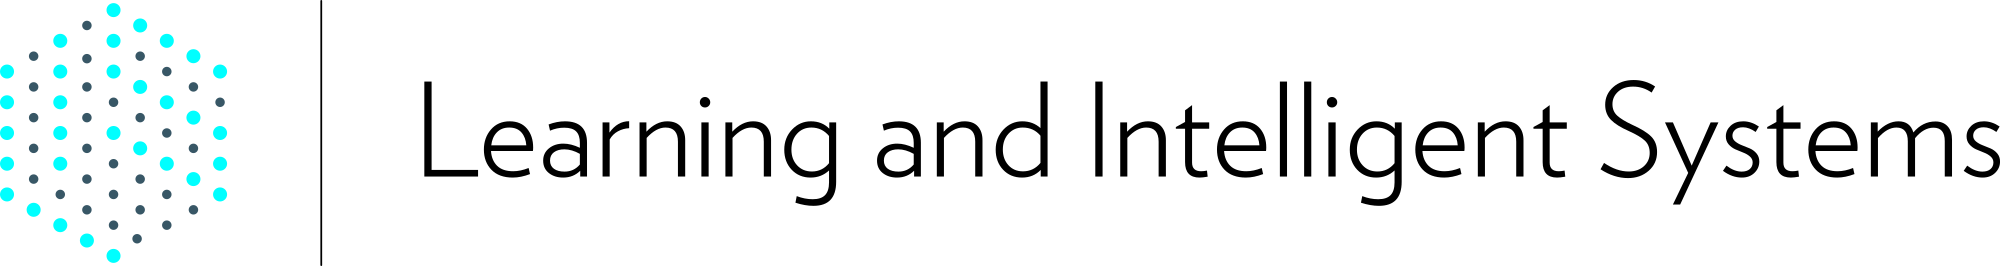
\includegraphics[height=.08\textwidth]{title/LIS-logo-line.png}
\end{minipage}
\todo{Logo}
Technische Universität Berlin\\

School IV - Electrical Engineering and Computer Science\\

Intelligent Multi-Robot Coordination Lab\\[8ex]


\large{Master Thesis}\\[1ex]
\begin{hsheadfont}

    \Huge Reinforcement Learning for Collaborative Transport of Cable Suspended
    Payloads with Multiple Multirotors\\[1 ex]
    
\end{hsheadfont}



\ \\[5ex]
\normalsize
presented by\\[2ex]
{\hsheadfont\LARGE Viktor Lorentz }\\[2ex]

Matr.-Nr.: 482024\\[1ex]
M.Sc. Computer Engineering
\\[3cm]
Date of submission: \today
\\[2cm]





  


\hsfont




\begin{minipage}[b]{0.25\textwidth}
\end{minipage}
\begin{minipage}[b]{0.4\textwidth}
    

    Supervisors:               \\
    \begin{hsheadfont}
    Khaled Wahba \\
    Dr. Sayantan Auddy \\
    \end{hsheadfont}
\end{minipage}
\begin{minipage}[b]{0.35\textwidth}
  

    Examiners:              \\
    \begin{hsheadfont}
    Prof. Dr. Wolfgang Hönig \\ 
    Prof. Dr. Marc Toussaint \\
    \end{hsheadfont}
\end{minipage}
\end{center}
    














\restoregeometry
